% !TeX root = ../libro.tex
% !TeX encoding = utf8



\setchapterpreamble[c][0.75\linewidth]{%
	\sffamily
  
    Las redes neuronales convolucionales es un caso particular de redes neuronales en las que entran en juego las capas de convolución. Estas redes se desarrollaron a finales del siglo pasado con el objetivo de reconocer objetos en imágenes. Poco a poco fueron ganando fama y popularidad dando un gran empuje a la visión por computador. La primera gran innovación en lo que respecta a estas redes fue protagonizada por Yann LeCun en 1990 con su propuesta LeNet. A partir de ahí comenzó una carrera por el desarrollo de estas redes. El fomento de la competitividad y la inversión que había en inteligencia artificial contribuyeron al avance de este área y surgieron grandes y prometedoras propuestas poco a poco. Destacamos las arquitecturas AlexNet (2012), creada por Alex Krizhevsky, Ilya Sutskever and Geoff Hinton. Poco después surgió ZF Net (Matthew Zeiler and Rob Fergus, 2013),GoogLeNet (2014) ,VGGN(Karen Simonyan and Andrew Zisserman, 2014),ResNet(Kaiming He et al., 2015). \\
    
    
    El propósito de este capítulo no es hacer una descripción detallada sobre este tipo de redes neuronales, si no más bien introducirlas al lector de tal manera que sea capaz de comprenderlas aunque no tenga conocimiento previo del tema. El capítulo comenzará con una breve introducción que expone el motivo por el que las redes neuronales prealimentadas no hacen de tan bien el trabajo destinado a las redes convolucionales. Después se explicará la operación fundamental que subyace dentro de estas redes, la convolución. Se verá la convolución para el caso de funciones continuas y discretas y se abordará en los casos unidimensionales y bidimensionales, tras lo se estudiará brevemente un ejemplo práctico. Tras entender esta importante operación, se introducirán los distintos tipos de capas presenten en estas redes, así pues se verán las capas convolucionales junto con algunas de sus propiedades, las capas de pooling, las capas de normalización y las totalmente conectadas. Se finalizará el capítulo con una explicación en cuanto a cómo diseñar una arquitectura para este tipo de redes.\\
    
    La principal referencia usada ha sido el contenido del libro \textit{Deep Learning Book} \cite{Goodfellow-et-al-2016} y el material proporcionado por la universidad de \href{http://cs231n.stanford.edu/}{Standford}
    
    
	\par\bigskip
}
\chapter{Redes Neuronales Convolucionales}\label{ch:CNN}

\newpage
\section{Introducción}

        En las redes neuronales, vimos que la información viaja a través de las capas ocultas desde la entrada hasta la salida y en donde las neuronas de una capa están totalmente conectadas a las neuronas de la anterior. Este tipo de redes neuronales, no presentan resultados deseados cuando se trabaja con imágenes. Supongamos una imagen de tamaño $(200,200,3)$, haciendo que la primera capa oculta tenga un total de $200 \cdot 200 \cdot 3 = 120000$ pesos. Pueden parecernos más o menos pocos en función de la capacidad hardware que tengamos, en cambio, las imágenes que usamos en la práctica, suelen ser mucho más grandes, haciendo que necesitemos millones y millones de pesos. Esto resulta un tanto inmanejable. \\
        
        Las redes neuronales convolucionales aprovechan el hecho de que la entrada es una estructura multidimensional y restringen la arquitectura de manera más sensata. En una red neuronal convolucional cuando se tratan imágenes las capas se disponen en una estructura de tres dimensiones (ancho, largo y profundidad). Además, las neuronas de una capa sólo estarán conectadas a una pequeña región de la capa anterior, en lugar de manera totalmente conectada y se irá reduciendo progresivamente la dimensión hasta llegar a la capa de salida, la cual tendrá una estructura unidimensional, es decir, de la forma $(1,1,depth)$. \\
        
        
\section{Operador Convolución}

    En el área de las matemáticas y en especial, en el campo del análisis funcional, una convolución es un operador el cual transforma dos funciones $f$ y $g$ en una tercera que en cierto sentido representa la magnitud en la que se superponen f y una versión trasladada e invertida de g. Demos una definición de convolución en la que las funciones $f$ y $g$ son funciones reales de variable real.
    
    \begin{definicion}[Convolución]\label{def:conv_1}
    Sean $f,g:\R \to \R$ dos funciones reales de variable real. Se define la convolución de $f$ y $g$, como 
    \begin{equation}
        (f*g)(t) = \int_{-\infty}^{\infty} f(x)g(t-x) \; dx
    \end{equation}
    \end{definicion}
    
    Una interpretación geométrica de la definición anterior es que la convolución expresa el área de $g$ que queda solapada por la función $f$ cuando $g$ se desplaza a través del eje de abcisas. Notamos que para aplicar la definición anterior a nivel práctico necesitamos de un sistema que sea continuo, lo cual no tendremos en nuestro caso por trabajar con señales temporales. Por lo que necesitamos una definición discreta de la convolución para el caso unidimensional.
    
    \begin{definicion}[Convolución Discreta Unidimensional]\label{def:conv_2}
    Sean $f,g:\mathbb{Z} \to \mathbb{Z}$ dos funciones con dominio y codominio en los enteros. Se define la convolución de $f$ y $g$ como
    \begin{equation}
        (f*g)(t) = \sum_{n \in \mathbb{Z}} f(n) g(t-n)
    \end{equation}
    \end{definicion}
    
    La definición de convolución discreta, así como la versión continua que dimos en \ref{def:conv_1} se puede extender a dimensión mayor. Por ejemplo, en imágenes se suelen trabajar con convoluciones $2$-dimensionales en la que la funciones $f$ y $g$ toman valores en $\mathbb{Z}\times\mathbb{Z}$ y la convolución se expresa como
    
    \begin{equation}\label{eq:conv_3}
        (f*g)(s,t) = \sum_{n \in \mathbb{Z}} \sum_{n \in \mathbb{Z}} f(n,m)g(s-n,t-m)
    \end{equation}



    En el contexto en el que aplicaremos esta operación, denotaremos a la función $f$ como $x$ la cual jugará el papel de \textit{entrada} (puede ser una imagen o una serie temporal) y a la función $g$ como $w$ y la llamaremos \textit{núcleo}, \textit{kernel} o \textit{filtro}. No nos vamos a meter en el terreno de la convolución y en todas las posibilidades que ofrece, solamente comentaremos que gracias a su propiedad conmutativa, podemos permutar las variables de $f$ y $g$. Por ejemplo, si trabajamos con la definición de convolución discreta unidimensional \ref{def:conv_2}, tenemos que
    
    \begin{equation}
        (x*w)(t) = \sum_{n \in \mathbb{Z}} x(t-n) w(n)
    \end{equation}

    \noindent si usamos la definición para el caso de dimensión $2$ dada por \eqref{eq:conv_3}, entonces tendríamos
    
    \begin{equation}
        (x*w)(s,t) = \sum_{n \in \mathbb{Z}} \sum_{n \in \mathbb{Z}} x(s-n,t-m)w(n,m)
    \end{equation}

    \noindent Esta nueva visión es algo más práctica, ya que podemos ver los cálculos  en términos de una expresión que actúa sobre todos los puntos de la entrada. Existe una operación similar a la convolución llamada correlación cruzada en la que la única diferencia es que en esta última no invierte el núcleo, de esta manera quedaría como 
    
    \begin{equation}
        (x*w)(t) = \sum_{n \in \mathbb{Z}} x(t+n) w(n)
    \end{equation}
    \noindent en el caso unidimensional, y 
    \begin{equation}
        (x*w)(s,t) = \sum_{n \in \mathbb{Z}} \sum_{n \in \mathbb{Z}} x(s+n,t+m)w(n,m)
    \end{equation}
    
    \noindent en el bidimensional. \\ 
    
    Esta operación la denotaremos igual que la convolución y en la práctica no distinguiremos cual estamos usando, ya que la red neuronal se dedica a aprender los pesos del kernel y si usa una u otra, solo le basta con invertir el núcleo. El motivo de presentar la correlación cruzada es que muchas librerías de aprendizaje la implementan en vez de la convolución por motivos de eficiencia. 
    
    
    \begin{ejemplo}[Ejemplo convolución]
    
    Veamos a continuación un ejemplo, para ello nos vamos a fijar en la imagen \ref{fig:ejemplo_conv}. Nuestra matriz de entrada es la matriz numérica bidimensional situada más a la izquierda de la fotografía y el kernel es la matriz $3\times 3$ situada a la derecha de la matriz de entrada. \\
    
    El proceso de convolución consiste superponer el núcleo en la imagen de entrada e ir calculando operaciones elementales (suma y multiplicación), tras ello, se desliza el kernel por la entrada y se vuelven a realizar los cálculos.
    
    \begin{figure}[H]
        \centering
        \includegraphics[scale=0.8]{img/convolucion.png}
        \caption{Ejemplo de convolución. \href{https://medium.com/@bdhuma/6-basic-things-to-know-about-convolution-daef5e1bc411}{Fuente}}
        \label{fig:ejemplo_conv}
    \end{figure}
    
    
    En una imagen de verdad, dependiendo de como sea el filtro, obtendriamos un resultado como en el de la imagen \ref{fig:ejemplo_conv2} en donde se ha aplicado el filtro derivada.
    
    \begin{figure}[H]
        \centering
        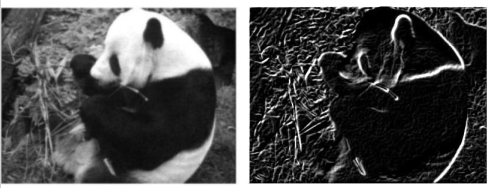
\includegraphics[scale=0.6]{img/ejemplo_conv2.png}
        \caption{(Izquierda) Imagen original. (Derecha) Imagen obtenida aplicando el filtro derivada}
        \label{fig:ejemplo_conv2}
    \end{figure}
    
    
    \end{ejemplo}
    
    
    La convolución es bastante útil porque presenta características clave que constribuyen a la mejora de un sistema de Machine Learning. 
    
    \begin{figure}[H]
        \centering
        \includegraphics[height=4cm, width=15cm]{img/redConv_1.png}
        \caption{(Izquierda) Una red neuronal con tres capas. (Derecha) Una red convolucional cuyas capas organizan las neuronas en tres dimensionas. Tal y como se visualiza, cada capa transforma el volumen de entrada $3$D en un volumen de salida también $3$D de las activaciones de las neuronas. La estructura rosa es la imagen de entrada.}
        \label{fig:red_conv_1}
    \end{figure}



\section{Capas usadas en redes convolucionales}

     \subsection{Capa convolucional}
  
        
        Una capa de convolución consiste en un conjunto de filtros que la red aprende. Cada filtro se extiende por la profundidad del volumen de la entrada. Durante la convolución deslizamos cada filtro a lo largo de la anchura y altura del volumen de entrada y calculamos los productos punto a punto entre las entre la imagen y el filtro. Al deslizar el filtro por la anchura y altura del volumen de entrada, producimos un mapa de salida bidimensional que da las respuesta de ese filtro en cada posición espacial. \\
        
        Intuitivamente, la red aprenderá filtros que se activan cuando ven algún tupo de característica visual como por ejemplo un borde o alguna mancha y conforme se va avanzando por la red estos patrones se volverán aún más complejos. Tendremos entonces un conjunto complejo de filtros en cada capa convolucional y cada uno de ellos producirá un capa de salida o activación bidimensional independiente. Se apilaran todos estos mapas a lo largo de la dimensión de profundidad dando lugar así al volumen de salida.  \\
        
        Comentemos a continuación los detalles de la conectividad de las neuronas, su organización en el espacio y su esquema de reparto de parámetros. \\
        
        \begin{center}
            \textbf{Disposición espacial}
        \end{center}
        
        La disposición espacial hace referencia a cuantas neuronas hay en el volumen de salida y a como están dispuestas. Hay tres hiperparámetros que controlan el tamaño de volumen de salida. La profundidad, la zancada y el zero-padding. \\
        
        La profundidad del volumen de salida corresponde al número de filtros que queremos usar, cada uno se especializa a buscar algo distinto en la entrada. Otro hiperparámetro es la zancada o paso, hace referencia a la zancada con la que deslizamos el filtro por la entrada. La zancada se mide por \textit{strides}. Un stride de uno indica que movemos el filtro unidad por unidad, en cambio, si es 3, entonces en cada deslizamiento, lo trasladamos tres posiciones. Así logramos volúmenes de salida más pequeños reduciendo así la dimensión espacial. Esto puede llegar a provocar la necesidad de rellenar el volumen de entrada con ceros alrededor del borde, el tamaño de este relleno también es otro hiperparámetro conocido como zero-padding. Se suele usar para preservar el tamaño espacial original del volumen de entrada. \\
        
        
        \begin{center}
            \textbf{Conectividad local}
        \end{center}
    
        Cuando las entradas presentan una alta dimensión, como por ejemplo el caso de imágenes, o series temporales con gran cantidad de canales sabemos que resulta poco útil conectar las neuronas todas con todas entre dos capas. En vez de ello, lo que se hace es conectar cada neurona a una región local del volumen de entrada. La extensión espacial de esta conectividad es un hiperparámetro que se llama \textit{campo receptivo} (que es el tamaño del filtro). La profundidad del filtro es siempre igual a la profundidad del volumen de la entrada. Es importante destacar que las conexiones son locales en cuanto a la anchura y a la altura, pero siempre son totales con respecto a la dimensión de profundidad del volumen de la entrada.
        
        \begin{ejemplo}
        Supongamos que tenemos un volumen de entrada de tamaño $(16,16,20)$ y usamos un filtro con un campo receptivo de $(3,3)$. Entonces cada neurona de la capa convolucional tendría entonces un total de $3*3*20 = 180$ conexiones al volumen de entrada. Notamos que la conectividad es local en el espacio bidimensional $anchura \times altura$ pero es total en cuanto a la profundidad, motivo por el cual, los filtro tienen profundidad $20$.
        \end{ejemplo}
        
        \begin{figure}[H]
            \centering
            \includegraphics[scale=0.5]{img/ejemplo_conv_3.png}
            \caption{(Izquierda) Un volumen de entrada en rojo y una capa convolucional con un volumen de neuronas. Cada neurona de esta capa está conectad a una sóla región local del volumen de entrada, pero a toda la profundidad. Notamos que en este caso hay 5 neuronas a lo largo de la profundidad de la capa, todas ellas están mirando a la misma región de la entada, es decir, comparten el mismo campo receptivo, pero eso no quiere decir que también compartan los pesos, ya que no es así. (Derecha) Las neuronas en las capas convolucionales no son distintas que las neuronas de las redes neuronales previamente estudiadas, estas siguen calculando un producto escalar de los pesos y la entrada, teniendo en cuenta el sesgo y pasando una función no lineal. \href{https://cs231n.github.io/convolutional-networks/}{Fuente}}
            \label{fig:ejemplo_conv_3}
        \end{figure}
        
        
        
        
        
        \begin{center}
            \textbf{Compartir parámetros}
        \end{center}
        
        El esquema de compartición de parámetros se usa para controlar el número de parámetros. Por lo general, si no tenemos esto en cuenta, vamos a tener millones de parámetro solo en la primera capa de la red convolucional. La verdad que es un número abrumadoramente alto teniendo en cuenta que lo habitual es que hayan varias capas. \\
        
        Resulta que se puede reducir drásticamente el número de parámetros haciendo una simple suposición: \textit{Si una característica es útil para calcular algo en una posición espacial $(x,y)$, entonces también debe de ser útil para calcular otra cosa en una posición $(x',y')$} Esto se traduce a que vamos a restringir a las neuronas a que usen los mismos pesos y sesgos fijada una profundidad. Así si tenemos un volumen de tamaño $(55,55,96)$, tenemos en particular $96$ niveles de profundidad y obligando a que en cada nivel hayan los mismos pesos, conseguimos reducir enormemente la cantidad de parámetros. \\
        
        Notamos que si todas las neuronas de un mismo nivel de profundidad usan el mismo vector de pesos, entonces la propagación hacia delante de la red puede calcularse en cada nivel de profundidad como una convolución de los pesos de la neurona con el volumen de entrada. Por ese motivo, se llaman capas convolucionales y también nos referimos, debido a de este mismo motivo, a los conjuntos de pesos como filtros o núcleos que se convoluciona con la entrada.\\
        
        Por último comentar que no siempre va a tener sentido realizar esta suposición. Por ejemplo, en el caso de imágenes de rostros centrados podría esperar que diferentes características específicas, como por ejemplo, los ojos o pestañas sean aprendidas en diferentes ubicaciones espaciales. En este caso es conveniente prescindir o relajar este esquema de compartición de parámetros y llamar a una capa totalmente conectada.
        
        
        \subsection{Capa de normalización} 
            Se han propuesto muchos tipos de capas de normalización para su uso en arquitecturas ConvNet, a veces con la intención de implementar esquemas de inhibición observados en el cerebro biológico. Sin embargo, estas capas han caído en desuso porque en la práctica se ha demostrado que su contribución es mínima, si es que hay alguna. 
        
        
        \subsection{Capas de Pooling}
        
        Es muy común usar de vez en cuando una capa de Pooling entre las sucesiva capas convolucionales. Esta capa se encarga de reducir progresivamente el tamaño espacial de la representación para conseguir una reducción significativa de la cantidad de parámetros y cálculos en la red y por tanto, controlar también así el sobreajuste. \\
        
        Esta capa opera de manea independiente en cada nivel de profundidad, pero aplica la misma operación a todos los niveles. Hay muchas maneras de aplicar pooling, la más frecuente es usar la técnica MAX-Pooling con filtros de tamaño $(2,2)$ aplicando un stride de $2$ que reduce la muestra de cada nivel de profundidad a lo largo de la anchura y profundidad.  Existen muchas más técnicas de pooling, como \textit{average-pooling} o \textit{L2-norm pooling}. En la imagen \ref{fig:ejemplo_conv_4} podemos observar un ejemplo. \\
        
        
        Actualmente hay una discusión en la comunidad investigadora sobre el empleo de esta capa, ya que algunos detractores piensan que pueden lograrse una reducción si la necesidad de emplearla aplicando sucesivas capas convolucionales con distintos strides y sin meter padding. Incluso también han demostrado empíricamente, que algunos modelos rinden mejor sin el empleo de estas capas. \\
        
        \begin{figure}[H]
            \centering
            \includegraphics[height=6cm, width=16cm]{img/ejemplo_conv_4.png}
            \caption{Ejemplo de capa de Pooling. Se opera por igual pero de manera independiente en todos los niveles de profundidad. (Izquierda)  El tamaño de la entrada es de $(224,224,64)$ y le aplicamos un pool con tamaño 2, y stride 2, por lo que el volumen inicial se reduce a $(112,112,64)$. Notamos que la profundidad no cambia. (Derecha)  La operación de downsampling más común es la del máximo, dando lugar a lo que se conoce como Max-Pooling. La imagen muestra un Max-Pooling con un stride de 2. Es decir, formamos bloques de $2 \times 2$ sobre de manera que no queden solapados (gracias a que el stride es igual a 2) y tomamos el máximo de dicho cuadrado como salida. \href{https://cs231n.github.io/convolutional-networks/}{Fuente}}
            \label{fig:ejemplo_conv_4}
        \end{figure}
        
        
        
        

        \subsection{Capas totalmente conectadas}
        
            Las neuronas de una capa totalmente conectada tienen conexiones completas con todas las salidas de la capa anterior, como se ve en las redes neuronales normales. Por lo tanto, sus salidas pueden calcularse con una multiplicación matricial seguida de una compensación de sesgo.\\
            
            La única diferencia entre las capas FC y CONV es que las neuronas de las segundas están conectadas a una sola región local de la entrada y muchas de ellas comparten parámetros. Sin embargo, el funcionamiento de las neuronas es el mismo en ambos casos resultando posible convertir una capa FC a CONV y viceversa. \\
            
            
        
    
    
\section{Arquitecturas}
    
    En el apartado anterior vimos los distintos tipos de capas que se suelen emplear en estas redes. Ahora vamos a ver cómo se suelen apilar para formar arquitecturas redes neuronales convolucionales. Escribiremos explícitamente la función de activación RELU como una capa más. \\
    
    La forma más habitual que suele tener una arquitectura de este tipos de redes es unas cuantas capas CONV-RELU apiladas, se sigue con algunas capas de POOL para reducir la dimensión y repetimos este patrón hasta que la imagen haya alcanzado un tamaño lo suficientemente pequeño. Entonces es cuando se suele añadir una transición a una capa totalmente conectada, FC y en ese momento, la red adquiere estructura de red neuronal prealimentada con capas FC-RELU. La última capa totalmente conectada contiene la salida. El patrón lo podemos resumir de la siguiente manera:
    
    \begin{equation}
        INPUT \to [[CONV \to RELU]^N \to POOL?]^M \to [FC \to RELU]^K \to FC 
    \end{equation}
    
    \noindent donde * indica la repetición, POOL? indica la capa opcional de pool y las constantes $N,M$ y $K$ suelen adquierir valores entre cero y tres.\\
    
    Existen muchas arquitecturas de redes neuronales convolucionales que alcanzaron un gran éxito y suelen ser muy empleadas por presentar buenos resultados, entre ellas destacamos LeNet, AlexNet, ZR NET, GoogleLeNet, VGGNet, ResNet, DenseNet entre otras. Las dos últimas, ResNet y DenseNet incluyen módulos residuales que favorecen el aprendizaje, pero no entraremos en más detalles. \\ 
        
        
    
\endinput






Patrones de capas
La forma más común de una arquitectura ConvNet apila unas cuantas capas CONV-RELU, las sigue con capas POOL, y repite este patrón hasta que la imagen se ha fusionado espacialmente a un tamaño pequeño. En algún momento, es común la transición a capas totalmente conectadas. La última capa totalmente conectada contiene la salida, como las puntuaciones de las clases. En otras palabras, la arquitectura ConvNet más común sigue el patrón: